% bs-Script
% Kapitel 1
%
In LV-Zyklus Systemtechnik werden verschiedene Arten von Systemen 
behandelt. Deshalb soll zunächst eine Klärung des Begriffs 
\emph{System} versucht werden. 
\section{Systembegriff}
Problemlösung mit Hilfe von Rechnern:
\begin{itemize}
\item   einfache Probleme $\to$ einfache, überschaubare Programme
\item   komplexe Probleme \\
	$\to$ Erarbeitung von Teillösungen, es entstehen Komponenten einer
	Gesamtlösung, die zusammenarbeiten müssen. \\
	$\Rightarrow$ System
\item   in DV-Systemen typisch: \\
	parallel ablaufende Aktivitäten auf verschiedenen technischen 
	Komponenten (Betriebsmittel)
\end{itemize}
\section{Informationsverarbeitende Systeme}
Informationsverarbeitende Systeme bestehen - hardware-technisch - gesehen aus einer Vielzahl 
von aktiven und passiven Komponenten:
\begin{itemize}
\item   {\em aktiv:} Prozessoren, Peripheriegeräte
\item   {\em passiv:} Speicher
\end{itemize}
Abbildung \ref {Beschreibungsebenen} zeigt die Beschreibungsebenen eines 
informationsverarbeitenden Systems.
\begin{figure}
%	\centerline{\epsfxsize=10cm\epsfysize=10cm\epsfbox{bild-1.epsf}}
    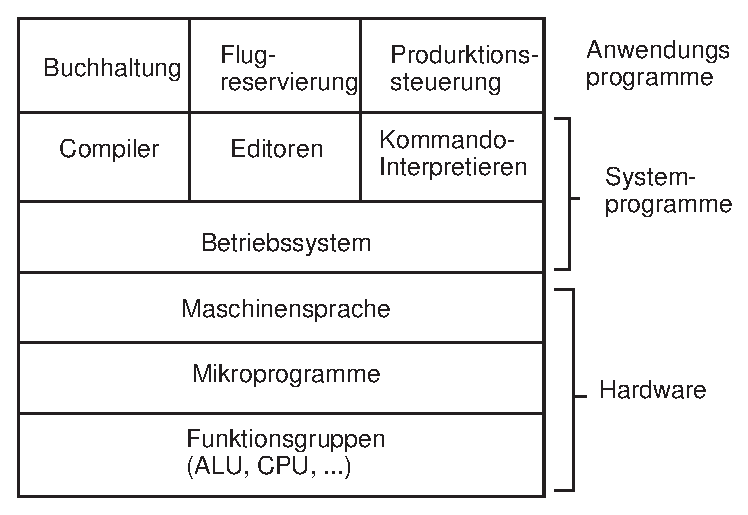
\includegraphics[scale=0.8]{bild-1.eps} %\centerline{\BoxedEPSF{bild-1.epsf  scaled 750}}
	\caption{\label{Beschreibungsebenen} Beschreibungsebenen eines informationsverarbeitenden Systems}
\end{figure}

Das Betriebssystem stellt die fundamentalste Komponente der 
Systemsoftware dar. 
Aufgaben, Strukturen und Prinzipien von Betriebssystemen finden sich in ähnlicher Form auch 
in anderen informationsverarbeitenden Systemen wieder (z.B. Datenbanksysteme, Flugbuchung, 
Produktionsüberwachung und -steuerung).

Architekturen von Betriebssystemen werden im folgenden stellvertretend für andere 
Systemarchitekturen betrachtet.

\paragraph{Erste grundlegende Aufgabe eines Betriebssystems:}
Bereitstellen einer virtuellen (abstrakten) Maschine, d.h. Befreiung des Programmierers
von Hardwaredetails. \\
\subparagraph{Beispiel:} Lesen eines Datenblocks von einer Festplatte  \\
Vorteile:
\begin{itemize}
\item   Drucken mit endlosem Papiervorrat
\item   fehlerfreie Datenübertragung
\end{itemize}
Nachteile:
\begin{itemize}
\item   u.U. nur unzureichende Unterstützung der Leistungsfähigkeit spezieller Geräte
(Beispiel: hochauflösender Grafikbildschirm wird zum Fernschreiber 
"`degradiert"')
\item   "`primitives"' Dateikonzept (vgl. z.B. PASCAL)
\end{itemize}
\paragraph*{Definition nach DIN 44300}
"`Betriebssystem ({\em operating system}): Die Programme eines digitalen Rechensystems,
die zusammen mit den Eigenschaften der Rechenanlage die Basis der möglichen Betriebsarten
des ditigalen Rechensystems bilden und insbesondere die Abwicklung von Programmen
steuern und überwachen. \\
Eine Sprache, der ein Betriebssystem gehorcht, heißt Betriebssprache ({\em operating language})."'
\paragraph{Zweite grundlegende Aufgabe eines Betriebssystems:}
Verwaltung der Betriebsmittel einer Rechenanlage \\
{\em Beispiele:} Druckerverwaltung, Speicherverwaltung

\section{Betriebssystemkategorien und Historie}
\paragraph{Rechner der ersten Generation}
(Röhren, 1945-1955) \\
Rechner der ersten Generation kannten keine Betriebssysteme.
Die Programmierung erfolgte durch Stecktafeln, später mit Lochkarten.
\paragraph{Rechner der zweiten Generation}
(Transistoren) \\
Programm- und Dateneingabe erfolgte mit Lochkarten, Ausgabe auf Drucker.
Es gab zwei Betriebsarten:
\begin{itemize}
\item   {\em online}-Betrieb
\item   {\em offline}-Betrieb (Puffern von Ein- und Ausgabe über Magnetbänder)
	sog. {\em Batch}-Systeme
\end{itemize}
Abbildung \ref{Batch-System} zeigt das Beispiel eines "`frühen"' 
Batch-Systems.

\begin{figure}
%	\centerline{\epsfxsize=10cm\epsfysize=10cm\epsfbox{bild-1.epsf}}
    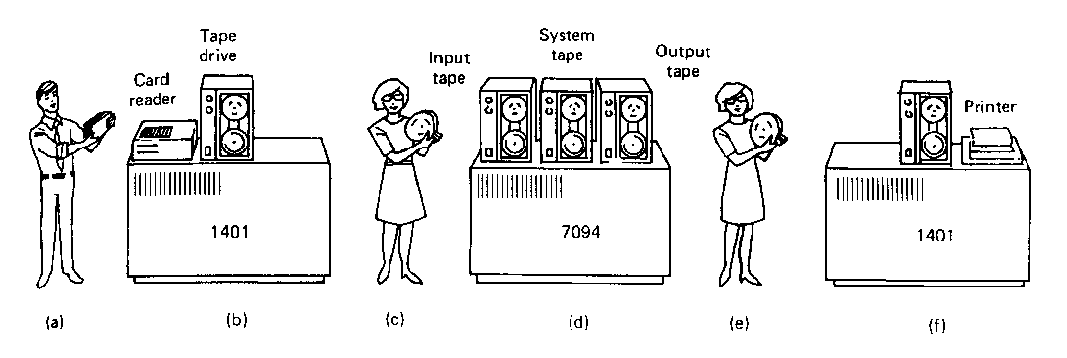
\includegraphics[scale=0.8]{bild-2.eps}%\centerline{\BoxedEPSF{bild-2.epsf  scaled 750}}
	\caption{\label{Batch-System} Batch-System, Bild entnommen aus 
	\cite{tanenbaum}}
\end{figure}

Die Ausführung eines sogenannten \emph{Batch-Jobs} umfaßte dabei die 
folgenden Schritte:
\begin{description}
	\item[(a)]  Programmierer liefert die Karten ab

	\item[(b)]  Vorrechner (IBM 1401) liest mehrere Benutzeraufträge (Jobs) 
	ein und schreibt sie auf ein Magnetband

	\item[(c)]  Operator legt Band in Station des Hauptrechners (IBM 7094) ein.

	\item[(d)]  Hauptrechner führt Benutzeraufträge aus und schreibt deren 
	Ausgabe auf ein weiteres Magnetband

	\item[(e, f)]  	Ausgabeband wird zum Vorrechner transportiert und Ergebnisse
	 werden dort ausgegeben.

\end{description}

Abbildung \ref{Batch-Job} zeigt ein Beispiel eines typischen Batch-Jobs.

\begin{figure}
%	\centerline{\epsfxsize=10cm\epsfysize=10cm\epsfbox{bild-1.epsf}}
    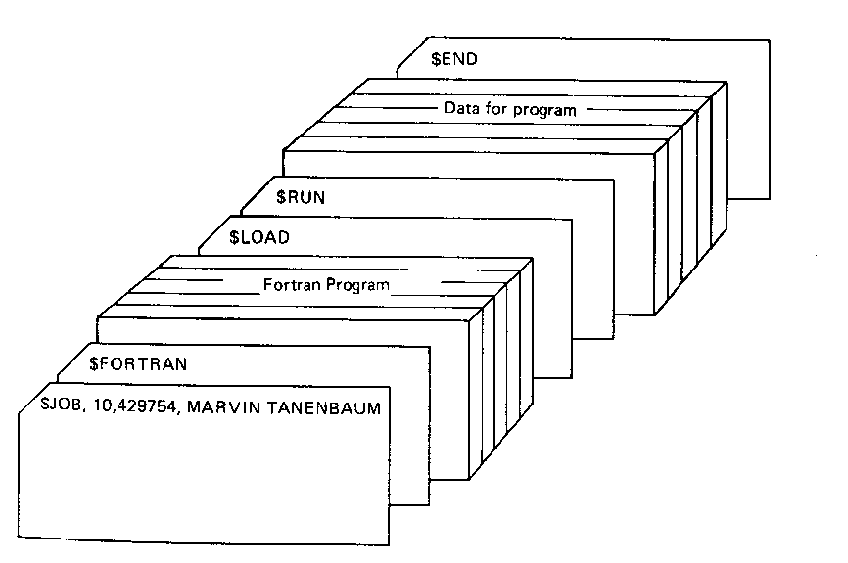
\includegraphics[scale=0.8]{bild-3.eps}%\centerline{\BoxedEPSF{bild-3.epsf  scaled 750}}
	\caption{\label{Batch-Job} Batch-Job als Kartenstapel, Bild entnommen aus 
	\cite{tanenbaum}}
\end{figure}

\paragraph{Einbenutzersystem im Einprogrammbetrieb} \ \\
Es gab drei Phasen der Job-Ausführung:
\begin{itemize}
\item   Programmeingabe
\item   Programmausführung
\item   Ergebnisausgabe
\end{itemize}
Für die folgenden Betrachtungen sollen für die Berechnung von
\emph{Prozessorauslastung} und \emph{Durchsatz} diese Formeln benutzt werden:
\begin{eqnarray*}
	\mbox{Prozessorauslastung} & = & \frac{\mbox{Ausführungszeit}}{\mbox{Verweildauer des Jobs in der Anlage}} \\
	\mbox{Durchsatz} & = & \frac{\mbox{Anzahl Jobs}}{\mbox{Zeiteinheit}}
\end{eqnarray*}
Beide Kenngrößen sind bei Terminal-Betrieb (wie z.B. durch einen Benutzer 
vor einer Workstation) beliebig schlecht, u.U. aber auch nicht von 
großer Bedeutung. Bei einem Betrieb mit Kartenleser und Drucker kann 
insbesondere die Eingabezeit drastisch vermindert werden. 

\subparagraph{Zahlenbeispiel:}
\begin{tabular}{ll}
	Eingabezeit (300 Karten): & 0,3 min. \\
	Ausgabezeit (500 Zeilen): & 0,5 min. \\
	Berechnungszeit: & 1 min.
\end{tabular}

Ausgehend von diesem Zahlenbeispiel zeigt die Tabelle in Abbildung 
\ref{Auslastung} in der linken Spalte mögliche Zeitangaben für die 
Durchführung des Benutzerauftrages im Online-Betrieb, d.h. die 
Rechenanlage steht dem Anwender für die Durchführung seines Jobs 
exklusiv zur Verfügung.

Betriebssysteme vor 1955 bestanden nur aus einen Einlese- und einem 
Druckprogramm. Eine weitergehende Bedienerunterstützung gab es nicht. 
Heute kann man sich solche Betreibssysteme nur leisten, wenn Auslastung 
und Durchsatz keine Rolle spielen (Personal Computer). Diesen Fall wollen 
wir vorerst nicht weiter betrachten.

Um eine Verbesserung von Durchsatz und Auslastung der damals teuren 
Hardware zu erzielen, entzog man den Rechner dem direkten Zugriff durch 
den Benutzer (closed-shop-Betrieb, offline). Dadurch konnte die Verweildauer eines 
Auftrags in der Anlage nahezu auf die Summe von Eingabezeit, Ausgabezeit 
und Berechnungszeit reduziert werden. Damit ergeben sich die in der 
rechten Spalte in Abbildung \ref{Auslastung} angegebenen Werte.
\begin{figure}
\begin{tabular}{l|l}
	{\em online}-Betrieb & {\em offline}-Betrieb \\
	\hline \\
	$\begin{array}{lcl}
		\mbox{Gesamtzeit} & = & 15 \mbox{ min.} \\
		\mbox{Prozessorauslastung} & = & \frac{1}{15} \approx 7\% \\
		\mbox{Durchsatz} & \approx & 4 \frac{\mbox{\small Jobs}}{h}
	\end{array}$
	&
	$\begin{array}{lcl}
		\mbox{Gesamtzeit} & = & 1.8 \mbox{ min.} \\
		\mbox{Prozessorauslastung} & = & \frac{1}{1.8} \approx 55\% \\
		\mbox{Durchsatz} & \approx & 33 \frac{\mbox{\small Jobs}}{h}
	\end{array}$
\end{tabular}	
\caption{\label{Auslastung} Prozessorauslastung und Durchsatz bei Online- und Offline-Betrieb}
\end{figure}

Voraussetzung für diesen Betrieb war, das die Ablaufsteuerung durch ein 
Betriebssystem vorgenommen wurde, daß sich ständig im Hauptspeicher 
befinden mußte. Damit entstanden gleichzeitig neue Probleme:
\begin{itemize}
	\item  Das Betriebssystem mußte gegen "`Angriffe"' durch die 
	 Benutzerprogramme geschützt werden.

	\item  Die Benutzerprogramme müssen nach Ablauf die Kontrolle an 
	das Betriebssystem zurückgeben.
\end{itemize}

\paragraph{Rechner der dritten Generation} (1965-1980)\\
waren u.a. gekennzeichnet durch:
\begin{itemize}
	\item  die Verwendung von Integrierte Schaltkreise (ICs, Chips)

	\item  die Benutzung sowohl für technisch-wissenschaftliche 
	(rechenintensive) und kommerzielle (E/A-intensive) Aufgaben
\end{itemize}
Typische Verteterin war die IBM 360 und ihre Nachfolger (370, 4300, 3080, 
3090). Das wichtigste zu lösende Problem war die  Verbesserung der 
Prozessorauslastung. Abbildung \ref{Beschaftigunglucken} zeigt 
exemplarisch die Zeitaufteilung zwischen dem Zentralprozessor und 
angeschlossenen Peripheriegeräten, die für die Abwicklung eines 
Programms benötigt werden.
\begin{figure}
\setlength{\unitlength}{5mm}
\begin{picture}(20,8)
	\put(0,6){CPU}
	\put(0,4){Gerät 1}
	\put(0,2){Gerät 2}
	\put(0,0){Gerät 3}
	\put(2,6){\line(1,0){2}}
	\put(4,6){\line(0,-1){2}}
	\put(4,4){\line(1,0){2}}
	\put(6,6){\line(0,-1){2}}
	\put(6,6){\line(1,0){2}}
	\put(8,6){\line(0,-1){4}}
	\put(8,2){\line(1,0){2}}
	\put(10,6){\line(0,-1){4}}
	\put(10,6){\line(1,0){2}}
	\put(12,6){\line(0,-1){6}}
	\put(12,0){\line(1,0){2}}
	\put(14,6){\line(0,-1){6}}
	\put(14,6){\vector(1,0){2}}
\end{picture}
	\caption{\label{Beschaftigunglucken} Aufteilung der Bearbeitungszeit 
	zwischen Prozessor und Peripheriegeräten}
\end{figure}
Die deutlich erkennbaren "`Beschäftigunglücken"' der CPU gaben Anlaß 
zu der grundlegenden Idee, diese Beschäftigunglücken für die 
ineinander verzahnte Bearbeitung mehrerer Aufträge zu nutzen, wie es in 
Abbilung \ref {Mehrprogrammbetrieb} dargestellt ist.
\begin{figure}
\begin{picture}(20,8)
	\put(0,6){CPU}
	\put(0,4){Gerät 1}
	\put(0,2){Gerät 2}
	\put(0,0){Gerät 3}
	\put(2,6){\line(1,0){2}}
	\put(4,6){\line(0,-1){2}}
	\put(4,4){\line(1,0){2}}
	\put(6,6){\line(0,-1){2}}
	\put(6,6){\line(1,0){2}}
	\put(8,6){\line(0,-1){4}}
	\put(8,2){\line(1,0){2}}
	\put(10,6){\line(0,-1){4}}
	\put(10,6){\line(1,0){2}}
	\put(12,6){\line(0,-1){6}}
	\put(12,0){\line(1,0){2}}
	\put(14,6){\line(0,-1){6}}
	\put(14,6){\vector(1,0){2}}
	\linethickness{0.5mm}
	\put(4,6){\line(1,0){1}}
	\put(5,6){\line(0,-1){6}}
	\put(5,0){\line(1,0){3.5}}
	\put(8.5,6){\line(0,-1){6}}
	\put(8.5,6){\line(1,0){1}}
	\put(9.5,6){\line(0,-1){2}}
	\put(9.5,4){\line(1,0){3}}
	\put(12.5,6){\line(0,-1){2}}
	\put(12.5,6){\line(1,0){1}}
	\put(13.5,6){\line(0,-1){4}}
	\put(13.5,2){\vector(1,0){2.5}}
\end{picture}
	\caption{\label {Mehrprogrammbetrieb} Mehrfachnutzung der CPU durch zwei 
	Programme}
\end{figure}

\paragraph{Mehrprogrammbetrieb} \ \\
Beim \emph{Mehrprogrammbetrieb} (\emph{Multiprogramming}) werden die 
Zeiten, während der die CPU auf die Fertigstellung einer E/A-Anforderung 
warten müßte, für die Bearbeitung eines anderen Benutzerauftrages 
genutzt. Dies ist nur unter der Vorraussetzung möglich, daß sich 
mehrere Programme (Benutzeraufträge) gleichzeitig im Hauptspeicher 
befinden. Abbildung \ref{Hauptspeicher} zeigt eine mögliche Aufteilung 
des Hauptspeichers.
\begin{figure}
\begin{picture}(10,12)
	\put(4,10){\framebox(8,1)[l]{\ Gerätesteuerung}}
	\put(4,8){\framebox(8,2)[l]{\ Betriebssystem}}
	\put(4,7){\framebox(8,1)[l]{\ Interrupt-Routine}}
	\put(4,5){\framebox(8,2)[l]{\ Benutzerauftrag 1}}
	\put(4,3){\framebox(8,2)[l]{\ Benutzerauftrag 2}}
	\put(4,1){\framebox(8,2)[l]{\ Benutzerauftrag 3}}
\end{picture}
	\caption{\label{Hauptspeicher} Aufteilung des Hauptspeichers bei 
	Mehrprogrammbetrieb}
\end{figure}

Beschränkung der Parallelarbeit ist im wesentlichen gegeben durch:
\begin{itemize}
\item   verfügbare Rechenzeit
\item   Platz im Hauptspeicher
\end{itemize}

Das Betriebssystem muß entscheiden können, zu welchen Zeitpunkten welcher
Benutzerauftrag bearbeitet wird. Unterbrechungen ({\em Interrupt}) des 
Zentralprozessors müssen ermöglicht werden. Bei jeder Unterbrechung  muß
ein Prozessorverwaltungsprogramm aufgerufen werden.
"`Langläufer"' müssen unterbrochen werden können (Zeitgeber).
\paragraph{Ziel:}
gerechte Verteilung der verfügbaren Prozessorzeit auf alle 
Benutzeraufträge \\
\bigskip
Unter \emph{Prozessen} sollen vorerst "`Träger parallel ablaufender 
Aktivitäten"' verstanden werden, die die CPU benötigen und selbst 
jeweils sequentiell ablaufen.

Aufgaben (und Probleme) des Betriebssystems:
\begin{enumerate}
\item   {\em Scheduling} (Prozessorverwaltung)
\item   gerechte Bedienung von Geräteanforderungen
\item   {\em Overhead}: Betriebssystem nimmt den Benutzeraufträgen Rechenzeit
 weg, diese benötigen daher mehr Zeit (Verweildauer im System)
\item   Schutz der Prozesse vor gegenseitigen Fehlfunktionen (seperater
 Adreßraum)
\item   Zugriffsrechte auf gemeinsam benutzte Daten verwalten
\item   Buchführung des Ressourcenverbrauchs
\item   "`{\em Spooling}"' (über Platten) der Job-Ein- und -Ausgabe
\end{enumerate}
Mehrprogrammbetriebssysteme mit Verdrängung beziehen auch Benutzeraufträge, die
sich z. Zt. nicht im Hauptspeicher befinden, in die Vergabeplanung von 
Betriebsmitteln ein. Dies führt zur Ein- und Auslagerung von Prozessen. 

\subparagraph{Interaktive Mehrbenutzersysteme im Mehrprogrammbetrieb:}
{\em Time-Sharing}-Be"-triebs"-sys"-teme
sind eine Weiterentwicklung des Mehrprogrammbetiebs, bei dem viele 
Benutzer über Terminals online mit der Rechenanlage verbunden sind. Als 
zusätzliche Aufgabe für das Betriebssystem entsteht die Forderung, 
jedem Benutzer durch geeignete Prozessorzuteilung den Eindruck zu 
vermitteln, die Rechenanlage würde nur für ihn arbeiten.

\paragraph{Rechner der vierten Generation}
(1980 - heute) \\

\bigskip
\textbf{Schlagworte:}
\begin{itemize}
	\item  Hardware
	\begin{itemize}
		\item  Höchstintegration (VLSI)
	
		\item  Personal Computer
	
		\item  Workstations
	\end{itemize}

	\item  Typische Betriebssysteme
		\begin{itemize}
		\item   MS-DOS (PC)
		\item   UNIX
		\item   MVS (IBM), VMS (digital)
		\end{itemize}
		
	\item Neuere Entwicklungen
		\begin{itemize}
		\item   Netzwerk-Betriebssysteme
		\item   verteilte Betriebssysteme
		\end{itemize}
\end{itemize}

\section{Zusammenfassung}

\begin{itemize}
\item   Betriebssysteme stellen virtuelle Maschinen mit virtuellen Befehlen
	(genannt Systemaufrufe, {\em system calls}) bereit. Sie erlauben
	Benutzerprogrammen, Dienstleistungen des Betriebssystems in Anspruch zu
	nehmen.
\item   Prozesse (Träger parallel ablaufender Aktivitäten) enthalten ein 
    Benutzer-
	oder Systemprogramm sowie alle für die Ausführung notwendigen Informationen
	(u.a. Befehlszählerstand, Registerinhalte, Adreßraum (Speicherabbild,
	{\em core-image})).
	\begin{itemize}
	\item   Prozeßverwaltung: Erzeugen, Beenden, Suspendieren von Prozessen
	\item   Betriebsmittelverwaltung: Hauptspeicherverwaltung, Prozessorverwaltung
	\end{itemize}
\item   Dateisystem: Verwaltung von Daten mit peripheren Speichermedien
\item   Benutzerverwaltung
\end{itemize}


